\documentclass[a4paper,12pt]{article}
\usepackage[utf8]{inputenc}
\usepackage[T2A]{fontenc}
\usepackage[russian]{babel}
\usepackage{amsmath,amssymb}
\usepackage{graphicx}
\usepackage{geometry}
\usepackage{cite}
\usepackage{color}
\usepackage{algorithm2e}
\geometry{left=25mm,right=25mm,top=25mm,bottom=25mm}

\begin{document}

% ----------------------- Титульный лист -----------------------
\begin{titlepage}
  \centering
  {\large Московский государственный университет имени М.\,В.\,Ломоносова\\
  Механико-математический факультет\\
  Кафедра вычислительной математики}\\[2cm]

  {\LARGE Курсовая работа}\\[1cm]
  {\Large \textbf{«Исследование критериев остановки нелинейных решателей при моделировании ненасыщенной фильтрации»}}\\[1.5cm]

  {\large Выполнил: студент Петрунников Тимур Максимович\\
  Научный руководитель: Ануприенко Денис Валерьевич, к.ф.-м.н., н.с. ИБРАЭ РАН, м.н.с. ИВМ РАН}\\[2cm]

  Москва, 2025
\end{titlepage}

\tableofcontents
\newpage

% ----------------------- Введение -----------------------
\section{Введение}
Фильтрация жидкости в пористой среде является ключевым процессом в гидрогеологии и инженерной практике. Фильтрацию необходимо моделировать при решении различных задач, связанных с объектами, затрагивающими подземные воды. Для объектов, расположенных в приповерхностной зоне, фильтрация описывается нелинейным уравнением Ричардса. Практические задачи требуют учитывать сложную форму областей и неоднородность параметров, что делает аналитические решения невозможными, и используется численное решение. При построении разностных схем возникают нелинейные уравнения относительно сеточных неизвестных, решаемые итерационными методами. Но подбор критериев остановки итераций не совсем понятен для пользователя.

Цель данной работы -- разработка решателя начально-краевых задач для одномерного уравнения Ричардса методом конечных объемов и изучение достаточных критериев остановки. В ходе работы решались следующие задачи:
\begin{itemize}
  \item изучить модель ненасыщенной фильтрации на основе уравнения Ричардса;
  \item освоить построение численных схем методом конечных разностей и методом конечных объемов (МКО);
  \item реализовать решатель для ненасыщенной фильтрации на основе МКО и неявной схемы по времени, для решения использовать метод простой итерации (МПИ);
  \item провести численные эксперименты и исследовать поведение критерия остановки МПИ в зависимости от сеточной дискретизации.
\end{itemize}
Результаты работы могут быть полезны для расчетчиков, занимающихся моделированием ненасыщенной фильтрации в соответствующих программных комплексах.

% ----------------------- Обзор литературы -----------------------
\section{Модель ненасыщенной фильтрации}
Рассматривается одномерная область $x\in[0,L]$ с пористой средой. Уравнение сохранения массы и закон Дарси приводят к так называемому уравнению Ричардса \cite{BearCheng}:
\begin{equation}\label{eq:ivp_richards_1d}
	\begin{cases}
		\textcolor{black}
		{
			\frac{\partial \theta(h)}{\partial t} + S(h)
		}
		s_{stor}(x)\frac{\partial h}{\partial t} - \frac{\partial}{\partial x}\left(
		\textcolor{black}{K_r(h)}
		K(x)\frac{\partial h}{\partial x}\right) = 0, ~~~~ x \in (0,L), ~ t\in(0, t_{\max})\\
		h(0,t) = H_0,~~h(L,t) = H_L,\\
		h(x,0) = H_{init}(x)
	\end{cases}
\end{equation}
где
\begin{itemize}
	\item $h$ -- напор воды, основная неизвестная;
	\item $\theta(h)$ -- влагосодержание, нелинейная функция \cite{Mualem}
	\item $S(h) = \theta(h)/\theta_s$ -- насыщенность;
	\item $K(x)$ -- коэффициент фильтрации;
	\item $K_r(h)$ -- относительная проницаемость, нелинейная функция \cite{VG};
	\item $s_{stor}(x)$ -- коэффициент упругой емкости.
\end{itemize}

Из-за зависимости относительной проницаемости и влагосодержания от напора, уравнение Ричардса является нелинейным. 

\section{Численное решение}
\subsection{Дискретизация}

Дискретизация выполняется на равномерной сетке. Построение разностных схем осуществлялось с помощью метода конечных объемов (МКО), который распространен для решения уравнений фильтрации в практических задачах. Здесь используется его одномерная версия. Для применения МКО удобно ввести понятие потока:

\begin{equation}
	q = -K_r(h)		K(x)\frac{\partial h}{\partial x},
\end{equation}

и переписать уравнение Ричардса в виде двух уравнений:
\begin{equation}
	\begin{cases}
			\frac{\partial \theta(h)}{\partial t} + S(h)
		s_{stor}(x)\frac{\partial h}{\partial t} + \frac{\partial q}{\partial x} = 0,\\
		q = -K_r(h)		K(x)\frac{\partial h}{\partial x}.
	\end{cases}
\end{equation}

Далее первое уравнение интегрируется по ячейке $[x_i, x_{i+1}] \equiv [ih, (i+1)h]$:

\begin{equation}
	\int_{x_i}^{x_{i+1}}\left[ \frac{\partial \theta(h)}{\partial h}
	\frac{\partial h}{\partial t} + S(h)s_{stor}(x)\frac{\partial h}{\partial t}
	+
	\frac{\partial q}{\partial x}
	\right]dx = 0.
\end{equation}
 Неизвестные напоры в МКО располагаются в центрах ячеек. Потоки при этом расположены разграничивающих узлах.
 
 По времени используется полностью неявная схема Эйлера. В таком случае уравнение далее принимает вид 
 
 \begin{equation}
 	\left[ \frac{\partial \theta(h^{n+1}_i)}{\partial h}
 	\frac{h_i^{n+1} - h_i^{n}}{\Delta t} + S(h_i^{n+1})s_{stor}(x)\frac{h_i^{n+1} - h_i^n}{\Delta t}
 	\right]\Delta x
 	+
 	q_{i+1}^{n+1} - q_i^{n+1} = 0.
 \end{equation}
 
 Потоки приближаются конечными разностями. При этом коэффициент фильтрации берется по формуле среднего гармонического, а для относительной проницаемости применяется противопотоковая аппроксимация (вычисляется $h_{upw}$ -- наибольшее из значений в соседних ячейках):
 
 \begin{equation}
 	q_i = \frac{2K_iK_{i-1}}{K_i + K_{i-1}}K_r(h_{upw})\frac{h_i - h_{i-1}}{\Delta x}.
 \end{equation}
 
 \subsection{Решение систем нелинейных уравнений}
 Как и исходное уравнение Ричардса, построенная с помощью МКО разностная схема, то есть система уравнений относительно сеточных неизвестных, является нелинейной. На самом деле, она является линейной системой с трехдиагональной матрицей, зависящей от решения:
 \begin{equation}
 	A(h)h = b(h).
 \end{equation}
 
 Поэтому ее можно решать так называемым методом простой итерации (МПИ) \cite{Celia1990}, то есть вычислять матрицу по старым значениям и находить новые решением линейной системы. Далее приводится алгоритм МПИ.
 
 	\begin{algorithm}[H]\label{alg:time_step_richards}
 	\SetAlgoLined
 	На входе: $h^n$ -- вектор напоров на предыдущем шаге (если шаг первый -- задано начальным условием)\;
 	$k = 0$\;
 	$h^{n+1} = h^n$\;
 	$converged = false$\;
 	\While{$k < 50$}{
 		Составить матрицу $A(h^{n+1})$\ и вектор правой части $b(h^{n+1})$\;
 		Вычислить $r^k = A(h^{n+1})h^{n+1} - b(h^{n+1})$\;
 		\If{$||r^k||_2 < \varepsilon_{abs} \text{~~или~~} ||r^k||_2 < \varepsilon_{rel}\cdot||r^0||_2$}{
 			$converged = true$\;
 			break\;
 		}
 		Решить систему $A(h^{n+1})h^{n+1} = b(h^{n+1})$ прогонкой\;
 		$k = k+1$\;
 	}
 	\eIf{$converged == true$}{
 		МПИ сработал\;
 		$h^n = h^{n+1}$\;
 	}
 	{
 		Выйти с сообщением об ошибке: не сошелся МПИ\;
 	}
 	\caption{Шаг неявной схемой с методом простой итерации для нелинейного уравнения Ричардса}
 \end{algorithm}
 
 Как видно, остановка итераций МПИ определяется относительным ($\varepsilon_{rel}$) и абсолютным ($\varepsilon_{abs}$) критериями остановки. При этом на практике часто бывает так, что с самой первой итерации невязка $r$ настолько мала, что завершить итерации по относительному критерию $\varepsilon_{abs}$, часто равному $10^{-5} - 10^{-4}$, не удается, и основную роль играет абсолютный критерий $\varepsilon_{abs}$. Однако подбор этого значения не всегда очевиден. В частности, при изменении параметров дискретизации значение этого параметра, требуемое для достижения приемлемой точности, может меняться. 


\section{Численные эксперименты}
Рассматривается модельная задача о втекании воды в сухую колонку. Граничные условия следующие: $H_0 = -8 м$, $H_L = 0.25 м$, начльное условие: $H_{init} = -8 м$. Значения коэффициентов: $s_{stor} = 10^{-6}$ м$^{-1}$, $K(x) = 7.96$ м/сут, параметры Ван Генухтена: $\theta_s = 0.368, \theta_r = 0.102, n = 2, \alpha = 33.5$. Время моделирования составляет 0.001 суток, $\Delta t$ = 0.0001 суток. Далее для разных сеток демонстрируется эффект использования грубого критерия остановки $\varepsilon_{abs} = 0.1$ по сравнению с $\varepsilon_{abs} = 10^{-7}$. 

\begin{figure}[ht] \centering
	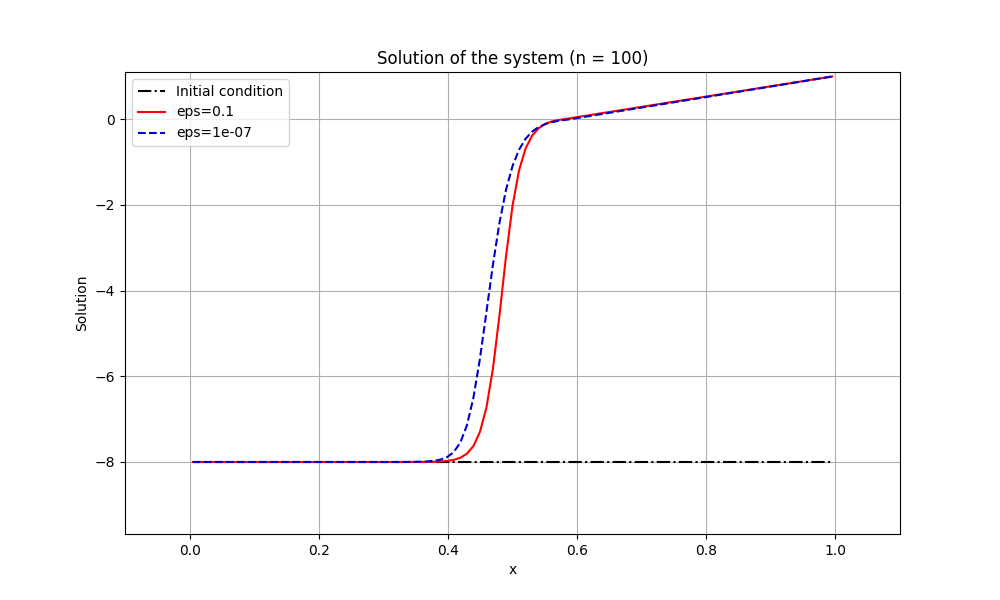
\includegraphics[width=\textwidth]{n100}
	\caption{Решения для $\varepsilon_{abs} = 0.1$, $\varepsilon_{abs} = 10^{-7}$ на сетке из 100 ячеек\label{pic:n100}}
\end{figure}

\begin{figure}[ht] \centering
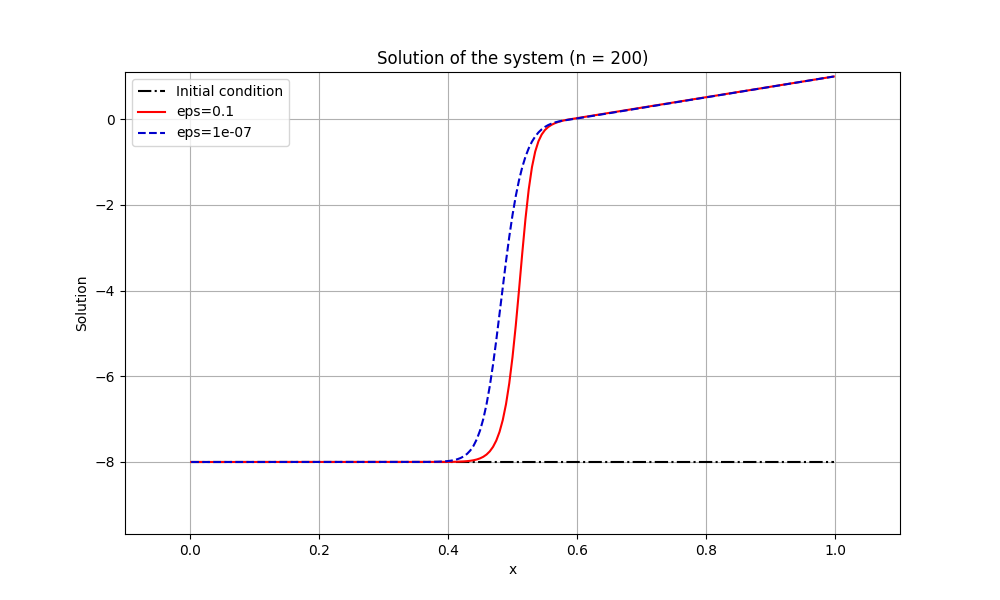
\includegraphics[width=\textwidth]{n200}
\caption{Решения для $\varepsilon_{abs} = 0.1$, $\varepsilon_{abs} = 10^{-7}$ на сетке из 200 ячеек\label{pic:n200}}
\end{figure}

\begin{figure}[ht] \centering
	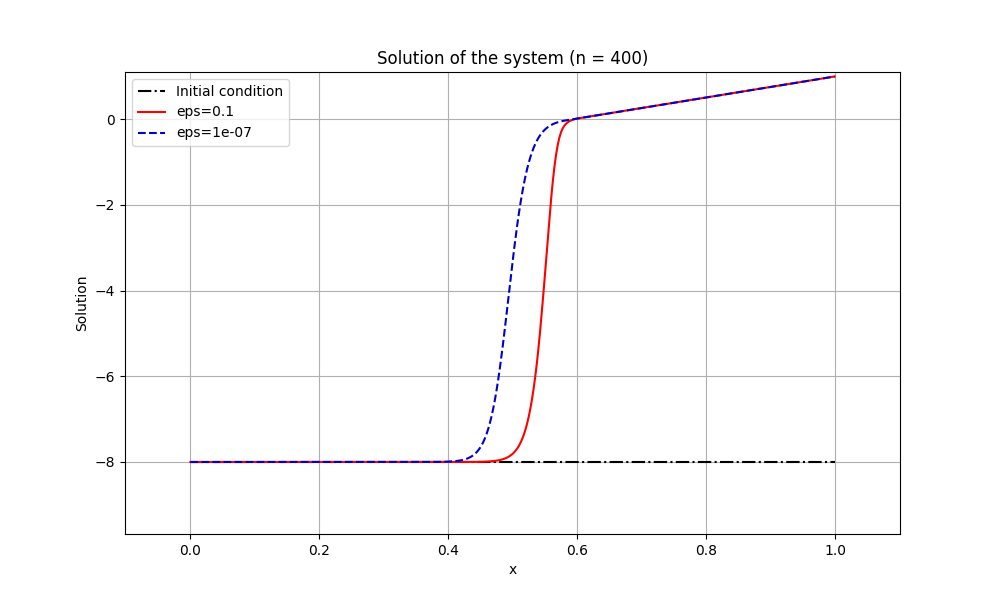
\includegraphics[width=\textwidth]{n400}
	\caption{Решения для $\varepsilon_{abs} = 0.1$, $\varepsilon_{abs} = 10^{-7}$ на сетке из 400 ячеек\label{pic:n400}}
\end{figure}

\begin{figure}[ht] \centering
	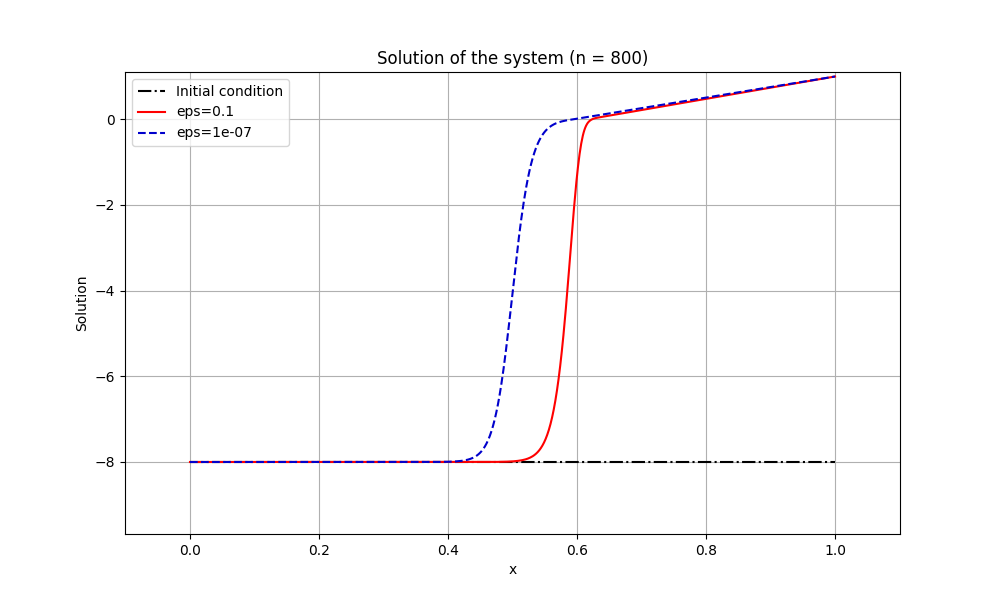
\includegraphics[width=\textwidth]{n800}
	\caption{Решения для $\varepsilon_{abs} = 0.1$, $\varepsilon_{abs} = 10^{-7}$ на сетке из 800 ячеек\label{pic:n800}}
\end{figure}

Решения, приведенные для сеток с 100, 200, 400 и 800 ячейками на рисунках \ref{pic:n100} -- \ref{pic:n800}, показывают, что при измельчении сетки положение фронта, полученного с грубым критерием остановки, все сильнее отстает от решения, полученного с более точным. Таким образом, для достаточного значения этого критерия, по-видимому, присутствует зависимость от дискретизации области.

% ----------------------- Заключение -----------------------
\section{Заключение}
Рассмотрена модель ненасыщенной фильтрации подземных вод на основе одномерного уравнения Ричардса. Для модели построена дискретизация с помощью метода конечных объемов и полностью неявной схемы Эйлера по времени. Для решения нелинейных систем используется метод простой итерации. Описанные методы программно реализованы на языке программирования Python. Проведенные численные эксперименты показали, что абсолютный критерий остановки метода простой итерации необходимо ужесточать с измельчением сетки. Полученная информация может быть полезна для расчетчиков, занимающихся моделированием ненасыщенной фильтрации.
% ----------------------- Библиография -----------------------
\begin{thebibliography}{9}
	\bibitem{BearCheng}
	Bear, Jacob, and Alexander H-D. Cheng. \textit{Modeling groundwater flow and contaminant transport}. Vol. 23. Dordrecht: Springer, 2010.
	
	\bibitem{Mualem}
	Mualem, Yechezkel. \textit{A new model for predicting the hydraulic conductivity of unsaturated porous media.} Water resources research 12.3 (1976): 513-522.
	
	\bibitem{VG}
	Van Genuchten, M. Th. \textit{A closed‐form equation for predicting the hydraulic conductivity of unsaturated soils.} Soil science society of America journal 44.5 (1980): 892-898.
	
\bibitem{Bear1972}
J. Bear. \emph{Dynamics of Fluids in Porous Media}. New York: Elsevier, 1972.

\bibitem{Celia1990}
M.\,A. Celia, E.\,T. Bouloutas, R.\,L. Zarba. A general mass-conservative numerical solution of Richards' equation. \emph{Water Resources Research}, 26(7):1483–1496, 1990.

\end{thebibliography}

% Чтобы отключить библиографию, закомментируйте блок \begin{thebibliography}...\end{thebibliography} 
% и удалите вызов пакета \usepackage{cite} при необходимости.

\end{document}
